\documentclass[11pt,a4paper]{article}

\usepackage[margin=25mm]{geometry}
\usepackage[T1]{fontenc}
\usepackage[utf8]{inputenc}
\usepackage{lmodern}
\usepackage{microtype}
\usepackage{amsmath,amssymb}
\usepackage{graphicx}
\usepackage{booktabs}
\usepackage{longtable}
\usepackage{array}
\usepackage{tabularx}
\usepackage{xcolor}
\usepackage{float}
\usepackage{caption}
\usepackage{subcaption}
\usepackage{fancyhdr}
\usepackage{enumitem}
\usepackage{hyperref}

\graphicspath{{figures/}}
\hypersetup{
  colorlinks=true,
  linkcolor=blue!45!black,
  citecolor=blue!45!black,
  urlcolor=blue!55!black,
  pdftitle={Explaining BERT Sentiment Predictions with Partition SHAP},
  pdfauthor={Mohsin Gourab}
}
\captionsetup{font=small,labelfont=bf}
\setlength{\parindent}{0pt}
\setlength{\parskip}{0.65em}
\setcounter{secnumdepth}{3}
\setcounter{tocdepth}{2}
\emergencystretch=2em

\pagestyle{fancy}
\fancyhf{}
\fancyhead[L]{BERT sentiment analysis with Partition SHAP}
\fancyhead[R]{TRDP II}
\fancyfoot[C]{\thepage}
\setlength{\headheight}{14pt}

\newcommand{\ResultSentenceCount}{10}
\newcommand{\ResultCorrectCount}{10}
\newcommand{\ResultMaxResidual}{0.00e+00}
\newcommand{\ResultMeanComp}{5.3107}
\newcommand{\ResultMeanSuff}{0.8927}
\newcommand{\ResultRuntime}{39.70}
\newcommand{\ResultModelEvaluations}{3,814}
\newcommand{\ResultForwardBatches}{253}


\newcommand{\sentenceplot}[3]{%
  \begin{figure}[p]
    \centering
    \includegraphics[width=\textwidth,height=0.79\textheight,keepaspectratio]{#1_word_shap.pdf}
    \caption{#2}
    \label{fig:#3}
  \end{figure}
}

\begin{document}

\hypersetup{pageanchor=false}
\begin{titlepage}
  \centering
  \vspace*{24mm}
  {\Large TRDP II\par}
  \vspace{16mm}
  {\huge\bfseries Explaining BERT Sentiment Predictions with Partition SHAP\par}
  \vspace{6mm}
  {\Large A token- and word-level analysis of an SST-2 classifier\par}
  \vspace{24mm}
  {\large Mohsin Gourab\par}
  \vfill
  \begin{minipage}{0.82\textwidth}
    \small
    This report documents the SHAP experiment implemented as a continuation of
    the earlier RFEM analysis. The original BERT checkpoint, sentence set, label
    convention, maximum sequence length, and masking principle were retained so
    that differences in the explanations arise from the attribution method rather
    than from a changed classifier.
  \end{minipage}
  \vfill
  {\large 23 September 2026\par}
\end{titlepage}

\hypersetup{pageanchor=true}
\pagenumbering{roman}
\begin{abstract}
This study applies Partition SHAP to a BERT classifier fine-tuned for binary
sentiment analysis. The experiment was motivated by the failure of an earlier
attention-based recursive feature elimination procedure to retain several
semantically important words. The classifier output explained here is the
difference between the positive and negative logits. A SHAP text masker creates
coalitions of available and unavailable tokenizer features; unavailable features
are represented by BERT's \texttt{[MASK]} token, and every perturbed sentence is
evaluated by the unchanged classifier. Token-level contributions are subsequently
aggregated over BERT WordPieces to obtain readable word-level explanations.

The evaluation used ten qualitative sentences carried over from the previous
experiment. The model classified all \ResultSentenceCount{} sentences correctly.
For every sentence, the SHAP base value plus the sum of the feature attributions
reconstructed the model margin, with a maximum stored additivity residual of
\(\ResultMaxResidual\). Masking the highest-ranked decision-supporting words
produced a mean comprehensiveness drop of \ResultMeanComp, while retaining only
those words produced a mean sufficiency gap of \ResultMeanSuff. The explanations
recover clear sentiment cues such as \emph{beautiful}, \emph{outstanding},
\emph{boring}, \emph{weak}, and \emph{captivating}. They also expose interaction-
dependent assignments that should not be read as context-free lexical sentiment.
\end{abstract}

\tableofcontents
\listoffigures
\listoftables
\clearpage
\pagenumbering{arabic}

\section{Introduction}

The previous TRDP experiment investigated whether an attention-derived recursive
feature elimination method could identify the words responsible for BERT's
sentiment decisions. That approach did not behave reliably: in several cases,
words carrying the clearest sentiment were assigned low importance or were removed
before less informative tokens. The present experiment therefore changes the
explanation method while leaving the predictive model and qualitative inputs
unchanged.

SHAP was selected because it defines feature attribution through changes in a
model output across coalitions of available features \cite{lundberg2017}. This is
substantively different from treating attention weights as feature importance.
For text, the relevant question is counterfactual: how does the classifier's
score change when a token or group of tokens is unavailable while other tokens
remain visible? Partition SHAP answers this question efficiently by respecting a
hierarchical clustering of features and estimating Owen-style values rather than
enumerating all \(2^M\) coalitions.

The objectives of the experiment are:

\begin{enumerate}[label=(\arabic*)]
  \item to obtain signed local attributions for each BERT tokenizer feature;
  \item to aggregate WordPiece attributions into readable word-level values;
  \item to verify the additive reconstruction of the explained classifier score;
  \item to test explanation faithfulness through comprehensiveness and sufficiency;
  \item to compare the resulting explanations with the qualitative behavior
        observed in the earlier RFEM study.
\end{enumerate}

\section{Model and explanation methodology}

\subsection{BERT sentiment classifier}

Let the input sentence be \(x\). BERT's tokenizer maps it to a sequence

\begin{equation}
  \tau(x) = (t_0,t_1,\ldots,t_{M+1}),
\end{equation}

where \(t_0=\texttt{[CLS]}\), \(t_{M+1}=\texttt{[SEP]}\), and the intervening
features may be complete words, punctuation, or WordPiece fragments. The
fine-tuned classifier returns two logits,

\begin{equation}
  \mathbf{z}_{\theta}(x)
  = \bigl(z_{\mathrm{NEG}}(x),z_{\mathrm{POS}}(x)\bigr).
\end{equation}

Class probabilities are obtained with the softmax function:

\begin{equation}
  p_{\theta}(y=c\mid x)
  = \frac{\exp\bigl(z_c(x)\bigr)}
         {\exp\bigl(z_{\mathrm{NEG}}(x)\bigr)
          +\exp\bigl(z_{\mathrm{POS}}(x)\bigr)}.
  \label{eq:softmax}
\end{equation}

The predicted class is \(\hat{y}=\arg\max_c p_{\theta}(y=c\mid x)\). The
checkpoint is \path{textattack/bert-base-uncased-SST-2}, which is based on the
BERT architecture \cite{devlin2019} and fine-tuned for the SST-2 task derived
from the Stanford Sentiment Treebank \cite{socher2013}. The implementation keeps
the previous TRDP label convention: index 0 is negative and index 1 is positive.

\subsection{Scalar target explained by SHAP}

SHAP requires the explained model to return a scalar for each perturbed input.
The wrapper therefore uses the signed logit margin

\begin{equation}
  f(x)=z_{\mathrm{POS}}(x)-z_{\mathrm{NEG}}(x).
  \label{eq:margin}
\end{equation}

A positive margin favors POS and a negative margin favors NEG. This choice also
fixes the sign convention of every attribution: \(\phi_i>0\) pushes the decision
toward positive sentiment, and \(\phi_i<0\) pushes it toward negative sentiment.
Using the logit margin avoids probability saturation and preserves the classifier's
unbounded evidence scale.

\subsection{Coalitions and the SHAP text masker}

For \(M\) explainable tokenizer features, a coalition is represented by a binary
vector \(\mathbf{m}\in\{0,1\}^{M}\). A value of one marks a feature as available;
a value of zero marks it as unavailable. The reconstruction function
\(h_x(\mathbf{m})\) maps the coalition to a perturbed sentence:

\begin{equation}
  h_x(\mathbf{m})_i =
  \begin{cases}
    t_i, & m_i=1,\\
    \texttt{[MASK]}, & m_i=0.
  \end{cases}
  \label{eq:masker}
\end{equation}

The corresponding coalition value is

\begin{equation}
  v_x(S)=f\!\left(h_x(\mathbf{1}_S)\right),
  \qquad S\subseteq\{1,\ldots,M\}.
  \label{eq:coalition-value}
\end{equation}

Consecutive mask tokens were not collapsed. This preserves tokenizer positions
and keeps the perturbation convention aligned with the earlier BERT experiment.
The \texttt{[CLS]} and \texttt{[SEP]} tokens remain part of model processing,
whereas punctuation and special tokens are excluded from content-word rankings.

\subsection{Shapley and Partition SHAP attribution}

For unrestricted coalitions, the Shapley value of feature \(i\) is the weighted
average of its marginal contribution over all subsets not containing \(i\):

\begin{equation}
  \phi_i =
  \sum_{S\subseteq N\setminus\{i\}}
  \frac{|S|!\,(M-|S|-1)!}{M!}
  \left[v_x(S\cup\{i\})-v_x(S)\right],
  \label{eq:shapley}
\end{equation}

where \(N=\{1,\ldots,M\}\). Exact evaluation is exponential in \(M\). The
Partition explainer instead builds a hierarchical feature tree \(\mathcal{T}\)
and evaluates coalitions consistent with that hierarchy. In permutation form,
the resulting Owen-style attribution may be written as

\begin{equation}
  \phi_i^{\mathcal{T}}
  =\frac{1}{|\Pi_{\mathcal{T}}|}
   \sum_{\pi\in\Pi_{\mathcal{T}}}
   \left[
     v_x\!\left(P_i^{\pi}\cup\{i\}\right)
     -v_x\!\left(P_i^{\pi}\right)
   \right],
  \label{eq:owen}
\end{equation}

where \(\Pi_{\mathcal{T}}\) is the set of hierarchy-consistent permutations and
\(P_i^{\pi}\) denotes the features preceding \(i\) in permutation \(\pi\). The
implementation allowed at most 500 model evaluations per sentence and processed
perturbations in batches of 32.

The local explanation is the additive model

\begin{equation}
  g(\mathbf{m})=\phi_0+\sum_{i=1}^{M}\phi_i m_i,
  \qquad \phi_0=v_x(\varnothing).
  \label{eq:additive-model}
\end{equation}

For the original sentence, local accuracy requires

\begin{equation}
  f(x)=\phi_0+\sum_{i=1}^{M}\phi_i.
  \label{eq:local-accuracy}
\end{equation}

The recorded additivity residual is

\begin{equation}
  \epsilon_{\mathrm{add}}
  =f(x)-\left(\phi_0+\sum_{i=1}^{M}\phi_i\right).
  \label{eq:additivity-residual}
\end{equation}

\subsection{WordPiece aggregation}

BERT may split a surface word into several WordPieces. If \(I_w\) is the set of
tokenizer positions belonging to word \(w\), its word-level attribution is the
signed sum

\begin{equation}
  \Phi_w=\sum_{i\in I_w}\phi_i.
  \label{eq:wordpiece}
\end{equation}

For example, the fragments \texttt{res}, \texttt{\#\#ili}, and
\texttt{\#\#ence} are displayed as \emph{resilience}. Summation preserves the
total contribution assigned to the original tokenizer features.

\subsection{Faithfulness measures}

Faithfulness was evaluated in the direction of the model's predicted class.
Define

\begin{equation}
  d=\begin{cases}
       +1, & \hat{y}=\mathrm{POS},\\
       -1, & \hat{y}=\mathrm{NEG},
     \end{cases}
  \qquad q(x)=d\,f(x).
  \label{eq:decision-score}
\end{equation}

Thus \(q(x)>0\) indicates support for the current prediction in both classes.
Words are ranked by \(d\Phi_w\). For a fraction \(\alpha\), the number of
selected words is

\begin{equation}
  k_{\alpha}=\max\!\left(1,\left\lceil \alpha W\right\rceil\right),
  \label{eq:selected-count}
\end{equation}

where \(W\) is the number of content-word groups. Let \(R_{\alpha}\) be the top
\(k_{\alpha}\) groups. Comprehensiveness measures how much the decision score
falls after those groups are masked:

\begin{equation}
  C_{\alpha}=q(x)-q\!\left(x\setminus R_{\alpha}\right).
  \label{eq:comprehensiveness}
\end{equation}

Higher \(C_{\alpha}\) indicates that the selected words were important for the
original prediction. The sufficiency gap measures the loss when only those words
remain visible:

\begin{equation}
  S_{\alpha}=q(x)-q\!\left(x_{R_{\alpha}}\right).
  \label{eq:sufficiency}
\end{equation}

Lower \(S_{\alpha}\) is preferred. Negative values can occur when the retained
subset supports the predicted class more strongly than the complete sentence.
These definitions follow the general rationale used in rationale evaluation
\cite{deyoung2020} while retaining the same text masker used by the explainer.

\subsection{Cross-sentence comparison}

The global plot is descriptive rather than a dataset-level global explanation.
For each word type \(w\) observed \(n_w\) times in the ten sentences, it reports

\begin{equation}
  G(w)=\frac{1}{n_w}\sum_{j=1}^{n_w}|\Phi_{w,j}|.
  \label{eq:global-importance}
\end{equation}

Absolute values are used because strong evidence for either class is important.

\section{Implementation workflow}

Figure~\ref{fig:workflow} summarizes the implemented path from the raw sentence
to word-level values. SHAP supplies coalitions to the text masker; the model
wrapper evaluates every resulting text under \texttt{torch.inference\_mode()},
and Partition SHAP combines the score differences. WordPiece aggregation takes
place only after token-level SHAP values have been computed.

\begin{figure}[H]
  \centering
  \fbox{%
    \begin{minipage}{0.82\textwidth}
      \centering\small
      Sentence \\
      $\downarrow$ \\
      BERT tokenizer $\rightarrow$ tokenizer features / WordPieces \\
      $\downarrow$ \\
      SHAP text masker $\rightarrow$ hierarchy-consistent coalitions \\
      $\downarrow$ \\
      Replace unavailable features with \texttt{[MASK]} \\
      $\downarrow$ \\
      BERT forward pass $\rightarrow$ logits $\rightarrow$
      \(z_{\mathrm{POS}}-z_{\mathrm{NEG}}\) \\
      $\downarrow$ \\
      Marginal contribution estimation $\rightarrow$ Partition SHAP values \\
      $\downarrow$ \\
      Sum WordPiece values $\rightarrow$ readable word-level SHAP values
    \end{minipage}%
  }
  \caption{Processing sequence followed by the implementation.}
  \label{fig:workflow}
\end{figure}

The implementation is divided into five source files. The model wrapper isolates
tokenization and inference; token aggregation handles feature alignment and
WordPiece joining; faithfulness evaluation applies ranked masks; plotting code
contains all visual output; and the run script coordinates configuration, I/O,
and execution. This separation made it possible to test model parity and SHAP
arithmetic independently of plotting and report generation.

\section{Experimental setup}

\subsection{Data}

The qualitative set contains ten manually specified sentences, denoted S1--S10.
Six have positive gold labels and four have negative gold labels. Several were
constructed to contain contrast or mixed evidence, including S3 (\emph{slow}
versus \emph{outstanding}) and S8 (\emph{weak} versus \emph{captivating}). The
complete set is reproduced in Appendix~\ref{app:sentences}.

\subsection{Configuration and reproducibility}

The run used Python 3.12.12, PyTorch 2.12.0, Transformers 5.9.0, SHAP 0.52.0,
NumPy 2.5.3, and Matplotlib 3.10.9 on CPU. Maximum sequence length was 128,
\texttt{max\_evals} was 500 per sentence, and the model evaluation batch size
was 32. Random seeds for NumPy and PyTorch were set to 42. The complete run took
\ResultRuntime{} seconds, evaluated \ResultModelEvaluations{} perturbed texts in
\ResultForwardBatches{} forward batches, and stored the configuration alongside
the numerical results.

\section{Results}

\subsection{Classification and additivity}

Table~\ref{tab:classification} reports the model decision and SHAP decomposition
for every sentence. All \ResultCorrectCount{} predictions agree with the gold
labels. The predicted-class probabilities exceed 0.999 for most examples; S2,
S3, S4, S7, S8, and S9 remain above 0.999 or close to it despite mixed wording in
some cases. These ten examples are qualitative probes, so the result should not
be interpreted as an estimate of held-out accuracy.

\begin{table}[htbp]
\centering
\caption{Sentence-level classification and SHAP additivity results.}
\label{tab:classification}
\small
\resizebox{\textwidth}{!}{%
\begin{tabular}{lccccrrrc}
\toprule
ID & Gold & Pred. & Correct & $p(\hat{y}\mid x)$ & $f(x)$ & $\phi_0$ & $\sum_i\phi_i$ & $\epsilon_{\mathrm{add}}$ \\
\midrule
S1 & POS & POS & 1 & 0.999738 & 8.2464 & 3.5955 & 4.6509 & 0.0e+00 \\
S2 & NEG & NEG & 1 & 0.999214 & -7.1473 & 2.6621 & -9.8094 & 0.0e+00 \\
S3 & POS & POS & 1 & 0.999055 & 6.9631 & 3.5955 & 3.3675 & 0.0e+00 \\
S4 & NEG & NEG & 1 & 0.999311 & -7.2796 & 2.6621 & -9.9416 & 0.0e+00 \\
S5 & POS & POS & 1 & 0.999716 & 8.1665 & 3.5995 & 4.5670 & 0.0e+00 \\
S6 & POS & POS & 1 & 0.999731 & 8.2199 & 2.6621 & 5.5579 & 0.0e+00 \\
S7 & NEG & NEG & 1 & 0.999366 & -7.3636 & 3.0872 & -10.4508 & 0.0e+00 \\
S8 & POS & POS & 1 & 0.999030 & 6.9375 & 3.5955 & 3.3420 & 0.0e+00 \\
S9 & NEG & NEG & 1 & 0.999217 & -7.1515 & 3.5955 & -10.7470 & 0.0e+00 \\
S10 & POS & POS & 1 & 0.999771 & 8.3806 & 3.5995 & 4.7811 & 0.0e+00 \\
\bottomrule
\end{tabular}}
\end{table}


The maximum absolute residual in Equation~\eqref{eq:additivity-residual} is
\(\ResultMaxResidual\) at the stored precision. This verifies that the saved
attributions correspond to the same scalar margin returned by the BERT wrapper.
It does not, by itself, establish that the masking baseline is linguistically
ideal or that every individual value has a context-free semantic interpretation.

\subsection{Dominant local attributions}

Table~\ref{tab:topwords} identifies the largest positive and negative word-level
attribution in each sentence. The signs refer to the POS-minus-NEG margin, not
to correctness. Thus a strongly negative value is supporting evidence when the
model predicts NEG.

\begin{table}[htbp]
\centering
\caption{Largest positive and negative word-level attributions in each sentence.}
\label{tab:topwords}
\begin{tabular}{lllll}
\toprule
ID & Gold & Prediction & Largest positive attribution & Largest negative attribution \\
\midrule
S1 & POS & POS & beautiful (+2.2569) & of (-0.1773) \\
S2 & NEG & NEG & and (+2.3351) & waste (-5.6937) \\
S3 & POS & POS & outstanding (+3.7479) & slow (-1.0241) \\
S4 & NEG & NEG & a (+0.3156) & dull (-4.0125) \\
S5 & POS & POS & brilliant (+4.0473) & the (-0.5056) \\
S6 & POS & POS & breathtaking (+1.8503) & emotion (-1.7249) \\
S7 & NEG & NEG & charm (+1.5548) & boring (-3.5674) \\
S8 & POS & POS & captivating (+4.7673) & weak (-3.8786) \\
S9 & NEG & NEG & a (+0.5032) & hollow (-3.6939) \\
S10 & POS & POS & entertaining (+2.8358) & to (-0.4039) \\
\bottomrule
\end{tabular}
\end{table}


The explanations capture the main contrastive cues. In S1, \emph{beautiful}
has a SHAP value of \(+2.2569\), followed by \emph{portrait} at \(+1.0118\) and
\emph{resilience} at \(+0.8187\). In S3, \emph{outstanding} contributes
\(+3.7479\), while \emph{slow} contributes \(-1.0241\). In S7,
\emph{boring} contributes \(-3.5674\) and \emph{devoid} contributes
\(-1.6886\). The strongest contrast occurs in S8: \emph{captivating} contributes
\(+4.7673\), \emph{delivers} contributes \(+2.1066\), and \emph{weak}
contributes \(-3.8786\). These results address the central problem observed with
RFEM: the explanation now assigns substantial magnitude to sentiment-bearing
content words rather than eliminating them as unimportant.

Not every attribution is lexically intuitive. In S7, \emph{or} receives a large
negative contribution, while \emph{charm} receives a positive contribution even
though the complete sentence is strongly negative. In S6, \emph{emotion} is
negative despite the positive prediction. Such values reflect conditional model
behavior under the chosen coalitions and masking baseline. They should be read
as local interaction-dependent allocations, not as a sentiment dictionary.

\subsection{Cross-sentence importance}

Figure~\ref{fig:global} ranks the twenty word types with the highest mean absolute
word-level SHAP magnitude. Because the experiment contains only ten sentences,
the plot summarizes this selected set and is not a population-level estimate.

\begin{figure}[htbp]
  \centering
  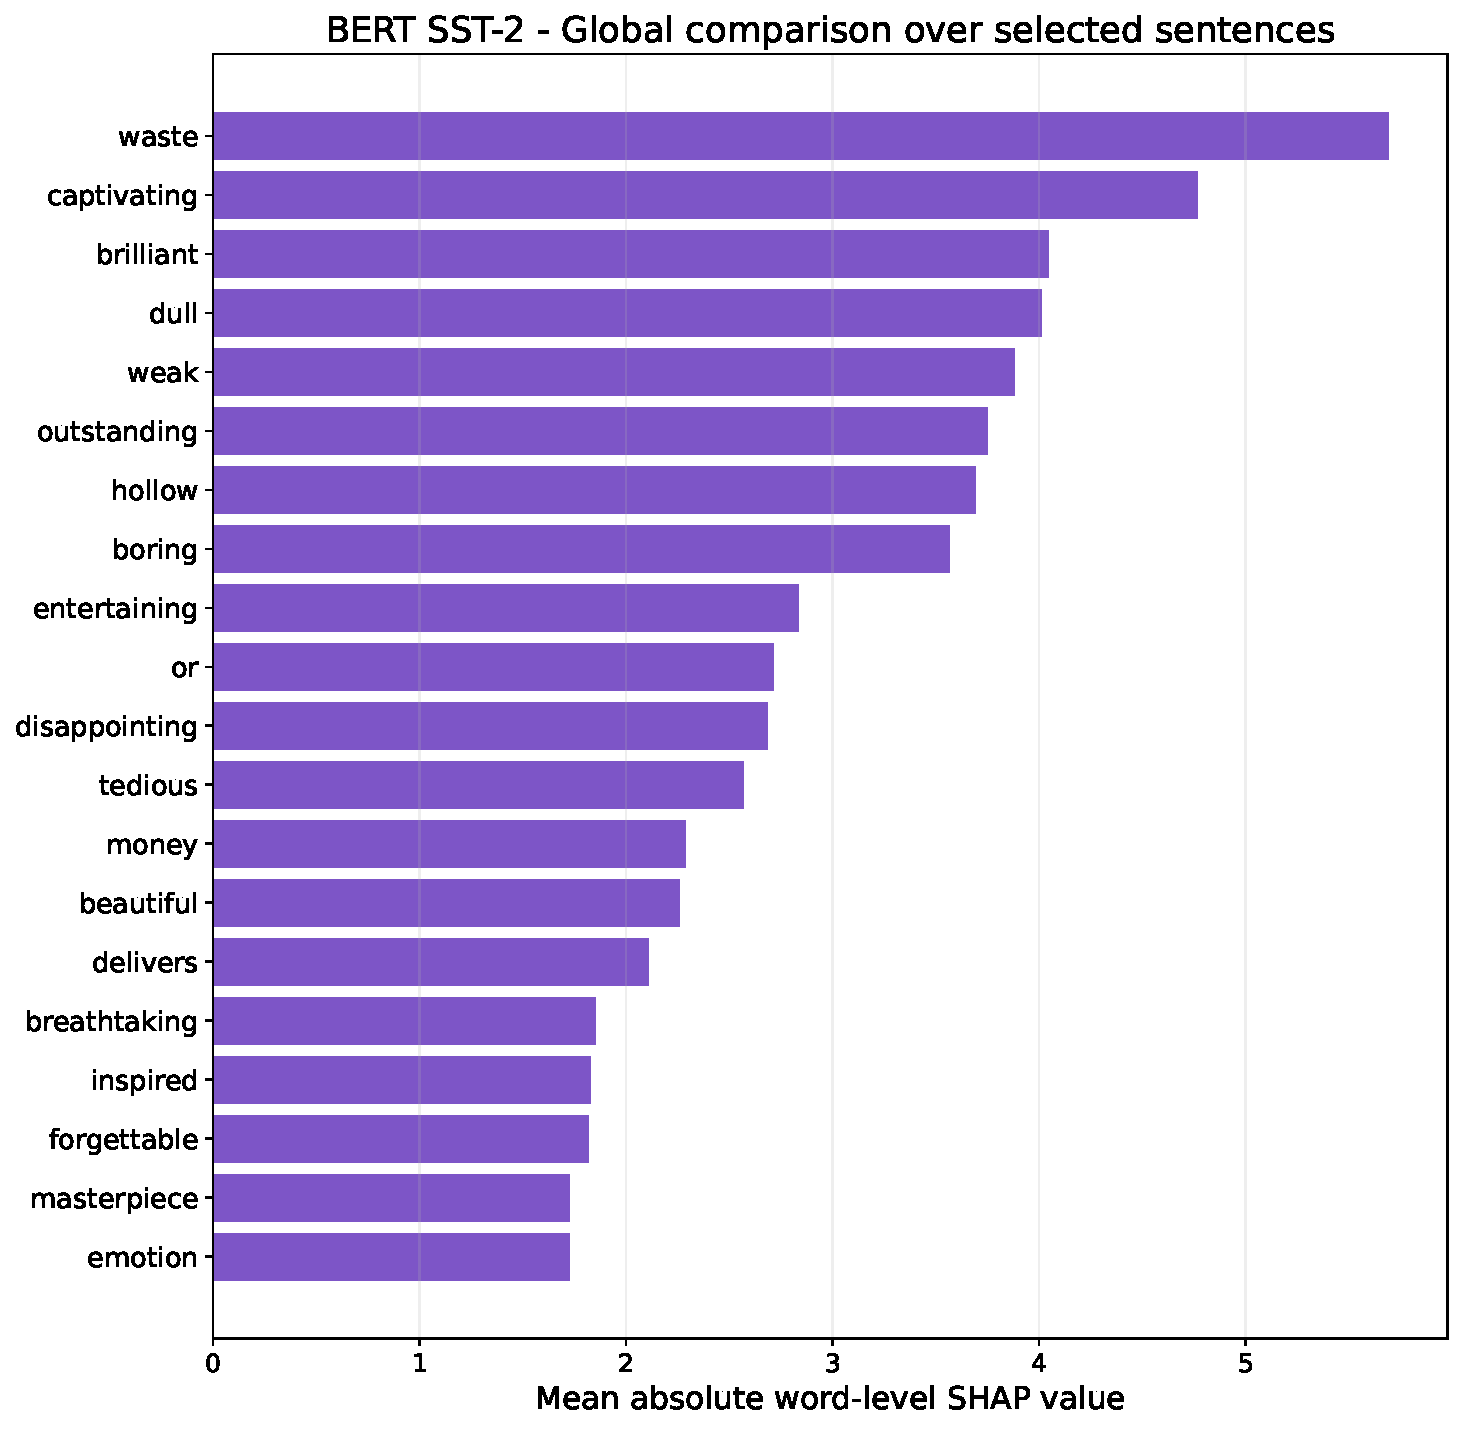
\includegraphics[width=0.88\textwidth]{global_mean_absolute_word_shap.pdf}
  \caption{Mean absolute word-level SHAP value over the ten qualitative sentences.}
  \label{fig:global}
\end{figure}

The largest magnitudes belong primarily to overt evaluative words, including
\emph{waste}, \emph{captivating}, \emph{brilliant}, \emph{outstanding},
\emph{hollow}, \emph{boring}, and \emph{dull}. This ordering is consistent with
the local plots, although averaging absolute values removes both sentence context
and attribution direction.

\subsection{Faithfulness}

Table~\ref{tab:faithfulness-aggregate} gives the mean faithfulness scores for
each selected fraction. Comprehensiveness increases as more highly ranked words
are removed, rising from approximately 2.38 at \(\alpha=0.1\) to 9.22 at
\(\alpha=0.5\). The sufficiency gap decreases from approximately 1.34 to 0.40 as
more words are retained. Both trends are consistent with the expected behavior
of a useful ranking.

\begin{table}[htbp]
\centering
\caption{Faithfulness results averaged over the ten sentences. Standard deviations are population standard deviations.}
\label{tab:faithfulness-aggregate}
\small
\begin{tabular}{crrrrr}
\toprule
Fraction $\alpha$ & Mean selected words & Mean comp. & SD comp. & Mean suff. gap & SD suff. gap \\
\midrule
0.1 & 1.50 & 2.3791 & 2.8969 & 1.3380 & 0.8157 \\
0.2 & 2.50 & 3.6865 & 3.8714 & 1.0390 & 0.4936 \\
0.3 & 3.50 & 5.9559 & 3.1109 & 0.7926 & 0.6147 \\
0.5 & 5.40 & 9.2213 & 2.6117 & 0.4013 & 0.6097 \\
\bottomrule
\end{tabular}
\end{table}


Across all forty fraction-sentence combinations, the mean comprehensiveness drop
is \ResultMeanComp{} and the mean sufficiency gap is \ResultMeanSuff{}. The
sentence-wise means in Table~\ref{tab:faithfulness-sentence} show that the
strength of this behavior varies across examples.

\begin{table}[htbp]
\centering
\caption{Mean faithfulness scores by sentence across $\alpha\in\{0.1,0.2,0.3,0.5\}$.}
\label{tab:faithfulness-sentence}
\begin{tabular}{lrr}
\toprule
ID & Mean comprehensiveness drop & Mean sufficiency gap \\
\midrule
S1 & 3.2323 & 1.2103 \\
S2 & 7.3672 & 0.8264 \\
S3 & 9.1041 & -0.1540 \\
S4 & 5.4999 & 0.6360 \\
S5 & 4.8566 & 0.9113 \\
S6 & 2.4668 & 1.4390 \\
S7 & 1.4940 & 1.5450 \\
S8 & 10.6432 & 0.3396 \\
S9 & 4.3473 & 0.8867 \\
S10 & 4.0954 & 1.2871 \\
\bottomrule
\end{tabular}
\end{table}


The detailed masks and scores are given in Appendix~\ref{app:faithfulness}. A
negative sufficiency gap in a few rows is not an error: it means that retaining
the selected subset increased the decision-direction score relative to the full
sentence, usually because conflicting evidence was removed.

\section{Discussion}

The SHAP experiment offers three improvements over the failed RFEM analysis.
First, it explains changes in an explicitly defined model output rather than
assuming that attention magnitude is equivalent to causal importance. Second,
it evaluates a feature in multiple coalition contexts, allowing interactions to
affect the final allocation. Third, it provides a direct additivity check and a
separate masking-based faithfulness evaluation.

The results nevertheless depend on methodological choices. The most important
choice is the missing-feature representation. BERT was fine-tuned on ordinary
SST-2 sentences, whereas the masker creates inputs containing one or more
\texttt{[MASK]} tokens. The classifier's behavior on those inputs may not match
its behavior on naturally occurring omissions. Partition SHAP also restricts
coalitions through a hierarchy; its values are Owen-style allocations and need
not match unrestricted exact Shapley values. Increasing the evaluation budget
reduces approximation variability but does not remove baseline dependence.

The sample is intentionally small and qualitative. It is suitable for inspecting
whether explanations recover known cues and handle contrastive examples, but it
cannot support claims about general explanation accuracy across SST-2. A larger
evaluation should include the SST-2 development set, perturbation baselines other
than \texttt{[MASK]}, repeated runs at several budgets, and comparisons with
alternative attribution methods such as Integrated Gradients.

\section{Conclusion}

Partition SHAP was successfully integrated with the existing BERT SST-2
classifier without changing the model, label mapping, or qualitative sentence
set. The method generated signed tokenizer-level explanations, preserved local
additivity for the POS-minus-NEG logit margin, and produced readable word-level
values through WordPiece aggregation. All ten predictions were correct, and the
main sentiment-bearing words generally received the largest attribution
magnitudes. Faithfulness scores changed in the expected direction as larger
fractions of the ranked words were removed or retained.

The experiment therefore provides a more defensible feature-attribution analysis
than the earlier attention-based elimination procedure. Its conclusions remain
local to the selected masker, model, and ten-sentence sample; the values should be
treated as model-behavior explanations under controlled perturbations rather than
as intrinsic linguistic properties of individual words.

\clearpage
\appendix

\section{Qualitative sentence set}
\label{app:sentences}
\begin{longtable}{@{}llp{0.73\textwidth}@{}}
\caption{Complete qualitative sentence set used in the experiment.}\label{tab:sentences}\\
\toprule
ID & Gold & Sentence \\
\midrule
\endfirsthead
\multicolumn{3}{l}{\tablename\ \thetable{} -- continued}\\
\toprule
ID & Gold & Sentence \\
\midrule
\endhead
\midrule\multicolumn{3}{r}{Continued on next page}\\
\endfoot
\bottomrule
\endlastfoot
S1 & POS & The film is a beautiful and moving portrait of human resilience. \\
S2 & NEG & This movie is an absolute waste of time and money. \\
S3 & POS & It's a bit slow at times but the performances are outstanding. \\
S4 & NEG & A dull, tedious and completely forgettable experience. \\
S5 & POS & The direction is inspired and the acting is nothing short of brilliant. \\
S6 & POS & A masterpiece of storytelling with breathtaking visuals and emotion. \\
S7 & NEG & Painfully boring and utterly devoid of any originality or charm. \\
S8 & POS & The screenplay is weak but the lead actor delivers a captivating turn. \\
S9 & NEG & A hollow and disappointing sequel that betrays everything the original stood for. \\
S10 & POS & Funny, heartfelt and endlessly entertaining from beginning to end. \\
\end{longtable}


\section{Complete sentence-level plots}
\label{app:plots}

The following figures reproduce every word-level plot produced by the verified
\texttt{modular\_s1\_s10} run. Red bars increase the POS-minus-NEG margin; blue
bars decrease it. The titles report the prediction, margin, base value, and
additivity residual.

\sentenceplot{S1}{Word-level Partition SHAP explanation for S1.}{S1}
\sentenceplot{S2}{Word-level Partition SHAP explanation for S2.}{S2}
\sentenceplot{S3}{Word-level Partition SHAP explanation for S3.}{S3}
\sentenceplot{S4}{Word-level Partition SHAP explanation for S4.}{S4}
\sentenceplot{S5}{Word-level Partition SHAP explanation for S5.}{S5}
\sentenceplot{S6}{Word-level Partition SHAP explanation for S6.}{S6}
\sentenceplot{S7}{Word-level Partition SHAP explanation for S7.}{S7}
\sentenceplot{S8}{Word-level Partition SHAP explanation for S8.}{S8}
\sentenceplot{S9}{Word-level Partition SHAP explanation for S9.}{S9}
\sentenceplot{S10}{Word-level Partition SHAP explanation for S10.}{S10}

\clearpage
\section{Complete word-level numerical results}
\label{app:word-values}
\small
\begin{longtable}{@{}lrlrrr@{}}
\caption{Complete word-level SHAP results. Support is signed in the direction of the predicted class.}\label{tab:word-values}\\
\toprule
ID & Index & Word & $\Phi_w$ & $|\Phi_w|$ & Prediction support \\
\midrule
\endfirsthead
\multicolumn{6}{l}{\tablename\ \thetable{} -- continued}\\
\toprule
ID & Index & Word & $\Phi_w$ & $|\Phi_w|$ & Prediction support \\
\midrule
\endhead
\midrule\multicolumn{6}{r}{Continued on next page}\\
\endfoot
\bottomrule
\endlastfoot
S1 & 0 & the & -0.142536 & 0.142536 & -0.142536 \\
S1 & 1 & film & 0.324253 & 0.324253 & 0.324253 \\
S1 & 2 & is & -0.160388 & 0.160388 & -0.160388 \\
S1 & 3 & a & 0.106850 & 0.106850 & 0.106850 \\
S1 & 4 & beautiful & 2.256860 & 2.256860 & 2.256860 \\
S1 & 5 & and & 0.208325 & 0.208325 & 0.208325 \\
S1 & 6 & moving & 0.598110 & 0.598110 & 0.598110 \\
S1 & 7 & portrait & 1.011846 & 1.011846 & 1.011846 \\
S1 & 8 & of & -0.177266 & 0.177266 & -0.177266 \\
S1 & 9 & human & -0.043383 & 0.043383 & -0.043383 \\
S1 & 10 & resilience & 0.818661 & 0.818661 & 0.818661 \\
S2 & 0 & this & -0.888101 & 0.888101 & 0.888101 \\
S2 & 1 & movie & -0.521932 & 0.521932 & 0.521932 \\
S2 & 2 & is & -0.775025 & 0.775025 & 0.775025 \\
S2 & 3 & an & 0.030125 & 0.030125 & -0.030125 \\
S2 & 4 & absolute & -0.775911 & 0.775911 & 0.775911 \\
S2 & 5 & waste & -5.693739 & 5.693739 & 5.693739 \\
S2 & 6 & of & -0.807296 & 0.807296 & 0.807296 \\
S2 & 7 & time & -0.259404 & 0.259404 & 0.259404 \\
S2 & 8 & and & 2.335107 & 2.335107 & -2.335107 \\
S2 & 9 & money & -2.285910 & 2.285910 & 2.285910 \\
S3 & 0 & it & -0.381619 & 0.381619 & -0.381619 \\
S3 & 1 & s & -0.348592 & 0.348592 & -0.348592 \\
S3 & 2 & a & -0.042201 & 0.042201 & -0.042201 \\
S3 & 3 & bit & -0.621683 & 0.621683 & -0.621683 \\
S3 & 4 & slow & -1.024147 & 1.024147 & -1.024147 \\
S3 & 5 & at & -0.046729 & 0.046729 & -0.046729 \\
S3 & 6 & times & -0.094758 & 0.094758 & -0.094758 \\
S3 & 7 & but & 0.741936 & 0.741936 & 0.741936 \\
S3 & 8 & the & 0.312652 & 0.312652 & 0.312652 \\
S3 & 9 & performances & 1.462643 & 1.462643 & 1.462643 \\
S3 & 10 & are & 0.177315 & 0.177315 & 0.177315 \\
S3 & 11 & outstanding & 3.747872 & 3.747872 & 3.747872 \\
S4 & 0 & a & 0.315643 & 0.315643 & -0.315643 \\
S4 & 1 & dull & -4.012466 & 4.012466 & 4.012466 \\
S4 & 2 & tedious & -2.570508 & 2.570508 & 2.570508 \\
S4 & 3 & and & -0.092597 & 0.092597 & 0.092597 \\
S4 & 4 & completely & -1.037591 & 1.037591 & 1.037591 \\
S4 & 5 & forgettable & -1.819339 & 1.819339 & 1.819339 \\
S4 & 6 & experience & 0.067303 & 0.067303 & -0.067303 \\
S5 & 0 & the & 0.050161 & 0.050161 & 0.050161 \\
S5 & 1 & direction & -0.451905 & 0.451905 & -0.451905 \\
S5 & 2 & is & -0.307505 & 0.307505 & -0.307505 \\
S5 & 3 & inspired & 1.829674 & 1.829674 & 1.829674 \\
S5 & 4 & and & 0.631725 & 0.631725 & 0.631725 \\
S5 & 5 & the & -0.505583 & 0.505583 & -0.505583 \\
S5 & 6 & acting & 0.210538 & 0.210538 & 0.210538 \\
S5 & 7 & is & -0.352823 & 0.352823 & -0.352823 \\
S5 & 8 & nothing & -0.320572 & 0.320572 & -0.320572 \\
S5 & 9 & short & 0.023784 & 0.023784 & 0.023784 \\
S5 & 10 & of & -0.374335 & 0.374335 & -0.374335 \\
S5 & 11 & brilliant & 4.047340 & 4.047340 & 4.047340 \\
S6 & 0 & a & 0.474689 & 0.474689 & 0.474689 \\
S6 & 1 & masterpiece & 1.726510 & 1.726510 & 1.726510 \\
S6 & 2 & of & 0.100716 & 0.100716 & 0.100716 \\
S6 & 3 & storytelling & 0.938018 & 0.938018 & 0.938018 \\
S6 & 4 & with & 0.399469 & 0.399469 & 0.399469 \\
S6 & 5 & breathtaking & 1.850310 & 1.850310 & 1.850310 \\
S6 & 6 & visuals & 0.190360 & 0.190360 & 0.190360 \\
S6 & 7 & and & 1.742435 & 1.742435 & 1.742435 \\
S6 & 8 & emotion & -1.724871 & 1.724871 & -1.724871 \\
S7 & 0 & painfully & -0.863948 & 0.863948 & 0.863948 \\
S7 & 1 & boring & -3.567362 & 3.567362 & 3.567362 \\
S7 & 2 & and & -0.352303 & 0.352303 & 0.352303 \\
S7 & 3 & utterly & -0.662267 & 0.662267 & 0.662267 \\
S7 & 4 & devoid & -1.688613 & 1.688613 & 1.688613 \\
S7 & 5 & of & -0.168164 & 0.168164 & 0.168164 \\
S7 & 6 & any & -1.480106 & 1.480106 & 1.480106 \\
S7 & 7 & originality & -0.275503 & 0.275503 & 0.275503 \\
S7 & 8 & or & -2.712506 & 2.712506 & 2.712506 \\
S7 & 9 & charm & 1.554754 & 1.554754 & -1.554754 \\
S8 & 0 & the & 0.080639 & 0.080639 & 0.080639 \\
S8 & 1 & screenplay & -0.485905 & 0.485905 & -0.485905 \\
S8 & 2 & is & -0.686718 & 0.686718 & -0.686718 \\
S8 & 3 & weak & -3.878561 & 3.878561 & -3.878561 \\
S8 & 4 & but & 0.449248 & 0.449248 & 0.449248 \\
S8 & 5 & the & 0.735832 & 0.735832 & 0.735832 \\
S8 & 6 & lead & 0.562615 & 0.562615 & 0.562615 \\
S8 & 7 & actor & 0.097387 & 0.097387 & 0.097387 \\
S8 & 8 & delivers & 2.106649 & 2.106649 & 2.106649 \\
S8 & 9 & a & 0.390013 & 0.390013 & 0.390013 \\
S8 & 10 & captivating & 4.767265 & 4.767265 & 4.767265 \\
S8 & 11 & turn & -0.654583 & 0.654583 & -0.654583 \\
S9 & 0 & a & 0.503179 & 0.503179 & -0.503179 \\
S9 & 1 & hollow & -3.693891 & 3.693891 & 3.693891 \\
S9 & 2 & and & -0.529555 & 0.529555 & 0.529555 \\
S9 & 3 & disappointing & -2.685714 & 2.685714 & 2.685714 \\
S9 & 4 & sequel & -0.816540 & 0.816540 & 0.816540 \\
S9 & 5 & that & -1.157125 & 1.157125 & 1.157125 \\
S9 & 6 & betrays & -0.827926 & 0.827926 & 0.827926 \\
S9 & 7 & everything & 0.131713 & 0.131713 & -0.131713 \\
S9 & 8 & the & -0.079131 & 0.079131 & 0.079131 \\
S9 & 9 & original & -0.256347 & 0.256347 & 0.256347 \\
S9 & 10 & stood & -1.091202 & 1.091202 & 1.091202 \\
S9 & 11 & for & -0.178729 & 0.178729 & 0.178729 \\
S10 & 0 & funny & 1.577193 & 1.577193 & 1.577193 \\
S10 & 1 & heartfelt & 0.803212 & 0.803212 & 0.803212 \\
S10 & 2 & and & 0.273088 & 0.273088 & 0.273088 \\
S10 & 3 & endlessly & 0.226613 & 0.226613 & 0.226613 \\
S10 & 4 & entertaining & 2.835799 & 2.835799 & 2.835799 \\
S10 & 5 & from & 0.083341 & 0.083341 & 0.083341 \\
S10 & 6 & beginning & 0.475263 & 0.475263 & 0.475263 \\
S10 & 7 & to & -0.403858 & 0.403858 & -0.403858 \\
S10 & 8 & end & -0.223215 & 0.223215 & -0.223215 \\
\end{longtable}

\normalsize

\clearpage
\section{Complete faithfulness results}
\label{app:faithfulness}
\small
\begin{longtable}{@{}lrrp{0.34\textwidth}rr@{}}
\caption{Complete faithfulness evaluation. Comp. is the comprehensiveness drop and suff. is the sufficiency gap.}\label{tab:faithfulness-detail}\\
\toprule
ID & $\alpha$ & $k$ & Selected words & Comp. & Suff. \\
\midrule
\endfirsthead
\multicolumn{6}{l}{\tablename\ \thetable{} -- continued}\\
\toprule
ID & $\alpha$ & $k$ & Selected words & Comp. & Suff. \\
\midrule
\endhead
\midrule\multicolumn{6}{r}{Continued on next page}\\
\endfoot
\bottomrule
\endlastfoot
S1 & 0.1 & 2 & beautiful | portrait & 0.9782 & 2.1121 \\
S1 & 0.2 & 3 & beautiful | portrait | resilience & 1.5693 & 1.4735 \\
S1 & 0.3 & 4 & beautiful | portrait | resilience | moving & 4.2399 & 0.8736 \\
S1 & 0.5 & 6 & beautiful | portrait | resilience | moving | film | and & 6.1418 & 0.3819 \\
S2 & 0.1 & 1 & waste & 4.3043 & 1.2533 \\
S2 & 0.2 & 2 & waste | money & 7.4392 & 0.9281 \\
S2 & 0.3 & 3 & waste | money | this & 7.2913 & 1.1335 \\
S2 & 0.5 & 5 & waste | money | this | of | absolute & 10.4340 & -0.0095 \\
S3 & 0.1 & 2 & outstanding | performances & 4.5409 & -0.0012 \\
S3 & 0.2 & 3 & outstanding | performances | but & 10.5901 & 0.1350 \\
S3 & 0.3 & 4 & outstanding | performances | but | the & 10.6039 & 0.0555 \\
S3 & 0.5 & 6 & outstanding | performances | but | the | are | a & 10.6815 & -0.8054 \\
S4 & 0.1 & 1 & dull & 0.2737 & 1.1605 \\
S4 & 0.2 & 2 & dull | tedious & 1.2735 & 0.8342 \\
S4 & 0.3 & 3 & dull | tedious | forgettable & 9.1523 & 0.3967 \\
S4 & 0.5 & 4 & dull | tedious | forgettable | completely & 11.3001 & 0.1528 \\
S5 & 0.1 & 2 & brilliant | inspired & 1.3549 & 0.6676 \\
S5 & 0.2 & 3 & brilliant | inspired | and & 1.8503 & 0.7298 \\
S5 & 0.3 & 4 & brilliant | inspired | and | acting & 5.2930 & 0.6618 \\
S5 & 0.5 & 6 & brilliant | inspired | and | acting | the | short & 10.9281 & 1.5858 \\
S6 & 0.1 & 1 & breathtaking & 0.3483 & 1.8376 \\
S6 & 0.2 & 2 & breathtaking | and & 0.4023 & 1.9966 \\
S6 & 0.3 & 3 & breathtaking | and | masterpiece & 3.2961 & 1.5983 \\
S6 & 0.5 & 5 & breathtaking | and | masterpiece | storytelling | a & 5.8204 & 0.3235 \\
S7 & 0.1 & 1 & boring & 0.2723 & 2.5498 \\
S7 & 0.2 & 2 & boring | or & 0.2553 & 1.0303 \\
S7 & 0.3 & 3 & boring | or | devoid & 0.9360 & 1.5410 \\
S7 & 0.5 & 5 & boring | or | devoid | any | painfully & 4.5125 & 1.0590 \\
S8 & 0.1 & 2 & captivating | delivers & 9.7611 & 0.3913 \\
S8 & 0.2 & 3 & captivating | delivers | the & 10.2428 & 0.6670 \\
S8 & 0.3 & 4 & captivating | delivers | the | lead & 10.0259 & -0.4161 \\
S8 & 0.5 & 6 & captivating | delivers | the | lead | but | a & 12.5431 & 0.7161 \\
S9 & 0.1 & 2 & hollow | disappointing & 1.7263 & 1.0374 \\
S9 & 0.2 & 3 & hollow | disappointing | that & 2.0574 & 1.0839 \\
S9 & 0.3 & 4 & hollow | disappointing | that | stood & 2.6488 & 1.3098 \\
S9 & 0.5 & 6 & hollow | disappointing | that | stood | betrays | sequel & 10.9568 & 0.1159 \\
S10 & 0.1 & 1 & entertaining & 0.2306 & 2.3713 \\
S10 & 0.2 & 2 & entertaining | funny & 1.1845 & 1.5115 \\
S10 & 0.3 & 3 & entertaining | funny | heartfelt & 6.0715 & 0.7724 \\
S10 & 0.5 & 5 & entertaining | funny | heartfelt | beginning | and & 8.8950 & 0.4932 \\
\end{longtable}

\normalsize

\clearpage
\section{Reproducibility record}

The independent implementation is stored under \path{bert_shap/}. Its principal
files are:

\begin{itemize}
  \item \path{config.json}: experiment defaults;
  \item \path{data/sentences.csv}: S1--S10 inputs and gold labels;
  \item \path{src/model_wrapper.py}: BERT inference and Equation~\eqref{eq:margin};
  \item \path{src/token_aggregation.py}: Equations~\eqref{eq:additivity-residual}
        and \eqref{eq:wordpiece};
  \item \path{src/evaluate_faithfulness.py}: Equations~\eqref{eq:comprehensiveness}
        and \eqref{eq:sufficiency};
  \item \path{src/make_comparison_plots.py}: sentence and global plots;
  \item \path{src/run_shap.py}: configuration, execution, and result writing;
  \item \path{tests/test_model_parity.py}: direct-model versus wrapper parity;
  \item \path{tests/test_additivity.py}: additive reconstruction and WordPiece tests.
\end{itemize}

Seven automated tests passed. The full modular run produced ten sentence rows,
104 word-level rows, forty faithfulness rows, and thirty-two plot/HTML artifacts.
The 104 word-level values were compared with the pre-refactor implementation and
matched exactly.

\begin{thebibliography}{9}

\bibitem{lundberg2017}
S. M. Lundberg and S.-I. Lee,
``A Unified Approach to Interpreting Model Predictions,''
\emph{Advances in Neural Information Processing Systems}, vol. 30, 2017.
\url{https://proceedings.neurips.cc/paper/2017/hash/8a20a8621978632d76c43dfd28b67767-Abstract.html}

\bibitem{devlin2019}
J. Devlin, M.-W. Chang, K. Lee, and K. Toutanova,
``BERT: Pre-training of Deep Bidirectional Transformers for Language Understanding,''
in \emph{Proceedings of NAACL-HLT}, pp. 4171--4186, 2019.
\url{https://aclanthology.org/N19-1423/}

\bibitem{socher2013}
R. Socher, A. Perelygin, J. Wu, J. Chuang, C. D. Manning, A. Ng, and C. Potts,
``Recursive Deep Models for Semantic Compositionality Over a Sentiment Treebank,''
in \emph{Proceedings of EMNLP}, pp. 1631--1642, 2013.
\url{https://aclanthology.org/D13-1170/}

\bibitem{deyoung2020}
J. DeYoung, S. Jain, N. F. Rajani, E. Lehman, C. Xiong, R. Socher, and B. C. Wallace,
``ERASER: A Benchmark to Evaluate Rationalized NLP Models,''
in \emph{Proceedings of ACL}, pp. 4443--4458, 2020.
\url{https://aclanthology.org/2020.acl-main.408/}

\bibitem{morris2020}
J. Morris, E. Lifland, J. Y. Yoo, J. Grigsby, D. Jin, and Y. Qi,
``TextAttack: A Framework for Adversarial Attacks, Data Augmentation, and
Adversarial Training in NLP,'' in \emph{Proceedings of EMNLP: System
Demonstrations}, pp. 119--126, 2020.
\url{https://aclanthology.org/2020.emnlp-demos.16/}

\bibitem{shapdocs}
SHAP documentation,
``Partition Explainer'' and ``Text Masker.''
\url{https://shap.readthedocs.io/}

\end{thebibliography}

\end{document}
